\documentclass[tikz]{standalone}

\usepackage{pgfplots}
\pgfplotsset{compat=1.16}

\begin{document}
    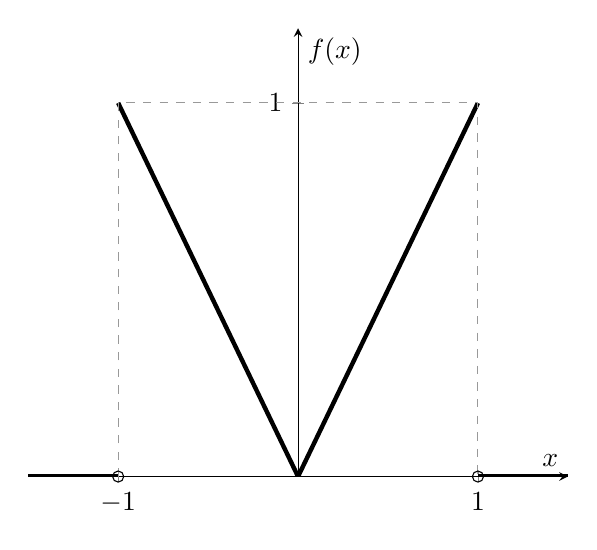
\begin{tikzpicture}
        % F(x)
        \begin{axis}[axis lines = center, xlabel = $x$, ylabel = {$f(x)$},ymax=1.2,ytick={1},xtick={-1,1}]
            \addplot[domain=-1.5:-1, samples=10,color=black, ultra thick]{0};
            \addplot[domain=-1:0, samples=10,color=black, ultra thick]{-x};
            \addplot[domain=0:1, samples=10,color=black, ultra thick]{x};
            \addplot[domain=1:1.5, samples=10,color=black, ultra thick]{0};
            \addplot[color=gray!80!white, style=dashed] coordinates{(-1,0)(-1,1)(1,1)(1,0)};
            \addplot[fill=white,mark=o] coordinates{(1,0)};
            \addplot[fill=white,mark=o] coordinates{(-1,0)};
        \end{axis}
    \end{tikzpicture}
    \begin{tikzpicture}
        % F(x)
        \begin{axis}[axis lines = center, xlabel = $x$, ylabel = {$F(x)$},ymax=1.2,ytick={1},xtick={-1,1}]
            \addplot[domain=-1.5:-1, samples=100,color=black, ultra thick]{0};
            \addplot[domain=-1:0, samples=100,color=black, ultra thick]{(1-x^2)/2};
            \addplot[domain=0:1, samples=100,color=black, ultra thick]{(1+x^2)/2};
            \addplot[domain=1:1.5, samples=100,color=black, ultra thick]{1};
            \addplot[color=gray!80!white, style=dashed] coordinates{(1,0)(1,1)};
            \addplot[color=gray!80!white, style=dashed] coordinates{(0,1)(1,1)};
        \end{axis}
    \end{tikzpicture}
\end{document}